\documentclass[12pt]{article}
\usepackage{graphicx}
\usepackage{subcaption}
\usepackage{amsmath}
\usepackage{amssymb}
\usepackage{amsfonts}

% Enter the specific assignment number and topic of that assignment below, and replace "Your Name" with your actual name.
\title{BIOS 611 Final Report - Cell Migration}
\author{Elizabeth Davis}
\date{\today}

\begin{document}
\maketitle
\begin{enumerate}
\item Figure 1
\begin{figure}[h!]
    \centering
    \begin{subfigure}[b]{0.4\linewidth}
      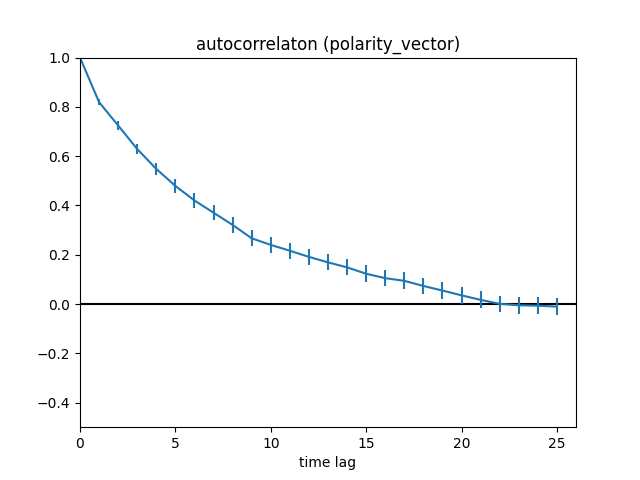
\includegraphics[width=\linewidth]{figures/acf_figures/glass_polarity_vector_acf_avg.png}
      \caption{Autocorrelation for polarity vector on glass}
    \end{subfigure}
    \begin{subfigure}[b]{0.4\linewidth}
      \includegraphics[width=\linewidth]{figures/acf_figures/stiff_polarity_vector_acf_avg.png}
      \caption{Autocorrelation for polarity vector on gel}
    \end{subfigure}
    \caption{These are different}
    \label{fig:acf_polvec}
  \end{figure}

\item Figure 2
\begin{figure}[h!]
    \centering
    \begin{subfigure}[b]{0.4\linewidth}
      \includegraphics[width=\linewidth]{figures/acf_figures/glass_polarity_angle_acf_avg.png}
      \caption{Autocorrelation for polarity angle on glass}
    \end{subfigure}
    \begin{subfigure}[b]{0.4\linewidth}
      \includegraphics[width=\linewidth]{figures/acf_figures/stiff_polarity_angle_acf_avg.png}
      \caption{Autocorrelation for polarity angle on gel}
    \end{subfigure}
    \caption{These are different}
    \label{fig:acf_polang}
  \end{figure}

\item Figure 3
\begin{figure}[h!]
    \centering
    \begin{subfigure}[b]{0.4\linewidth}
      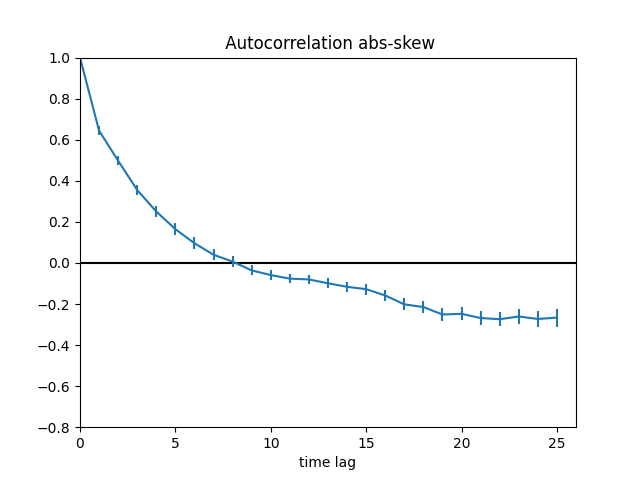
\includegraphics[width=\linewidth]{figures/acf_figures/glass_abs_skew_acf_avg.png}
      \caption{Autocorrelation for abs-skew on glass}
    \end{subfigure}
    \begin{subfigure}[b]{0.4\linewidth}
      \includegraphics[width=\linewidth]{figures/acf_figures/stiff_abs_skew_acf_avg.png}
      \caption{Autocorrelation for abs-skew on gel}
    \end{subfigure}
    \caption{These are different}
    \label{fig:acf_absskew}
  \end{figure}

\item Figure 4
\begin{figure}[h!]
    \centering
    \begin{subfigure}[b]{0.4\linewidth}
      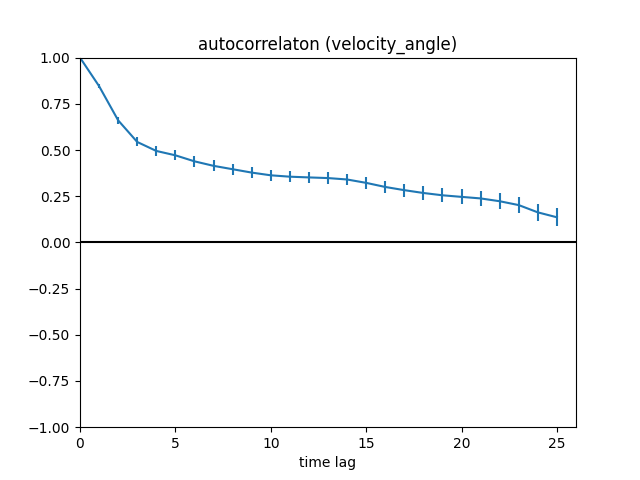
\includegraphics[width=\linewidth]{figures/acf_figures/glass_velocity_angle_acf_avg.png}
      \caption{Autocorrelation for velocity angle on glass}
    \end{subfigure}
    \begin{subfigure}[b]{0.4\linewidth}
      \includegraphics[width=\linewidth]{figures/acf_figures/stiff_velocity_angle_acf_avg.png}
      \caption{Autocorrelation for velocity angle on gel}
    \end{subfigure}
    \caption{These are different}
    \label{fig:acf_velang}
  \end{figure}

\item Figure 5
\begin{figure}[h!]
    \centering
    \begin{subfigure}[b]{0.4\linewidth}
      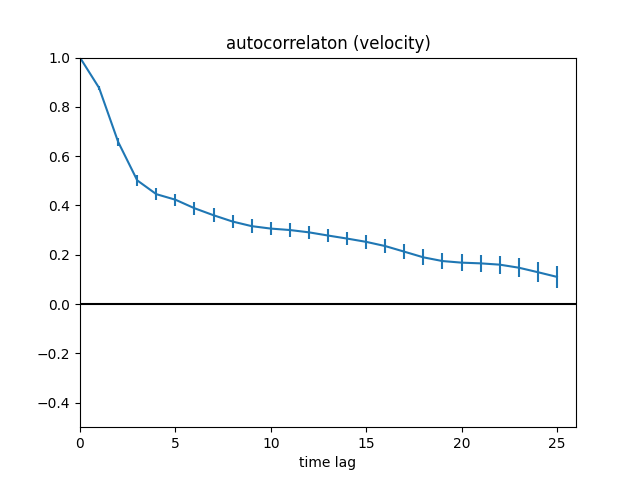
\includegraphics[width=\linewidth]{figures/acf_figures/glass_velocity_acf_avg.png}
      \caption{Autocorrelation for velocity on glass}
    \end{subfigure}
    \begin{subfigure}[b]{0.4\linewidth}
      \includegraphics[width=\linewidth]{figures/acf_figures/stiff_velocity_acf_avg.png}
      \caption{Autocorrelation for velocity on gel}
    \end{subfigure}
    \caption{These are different}
    \label{fig:acf_vel}
  \end{figure}

\item Figure 6
\begin{figure}[h!]
    \centering
    \begin{subfigure}[b]{0.4\linewidth}
      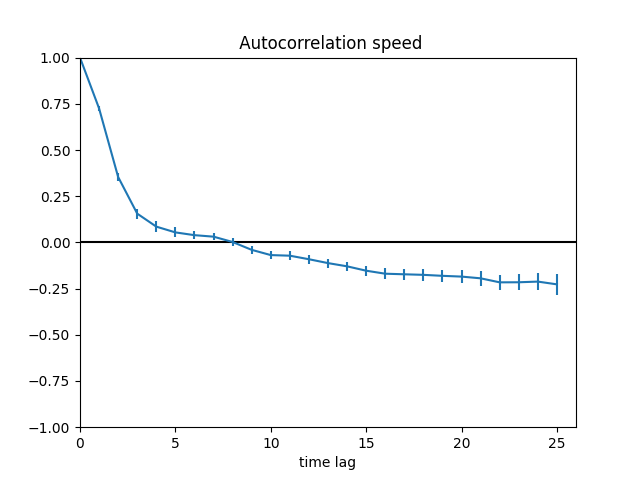
\includegraphics[width=\linewidth]{figures/acf_figures/glass_speed_acf_avg.png}
      \caption{Autocorrelation for speed on glass}
    \end{subfigure}
    \begin{subfigure}[b]{0.4\linewidth}
      \includegraphics[width=\linewidth]{figures/acf_figures/stiff_speed_acf_avg.png}
      \caption{Autocorrelation for speed on gel}
    \end{subfigure}
    \caption{These are different}
    \label{fig:acf_speed}
  \end{figure}

\item Figure 7
\begin{figure}[h!]
    \centering
    \begin{subfigure}[b]{0.4\linewidth}
      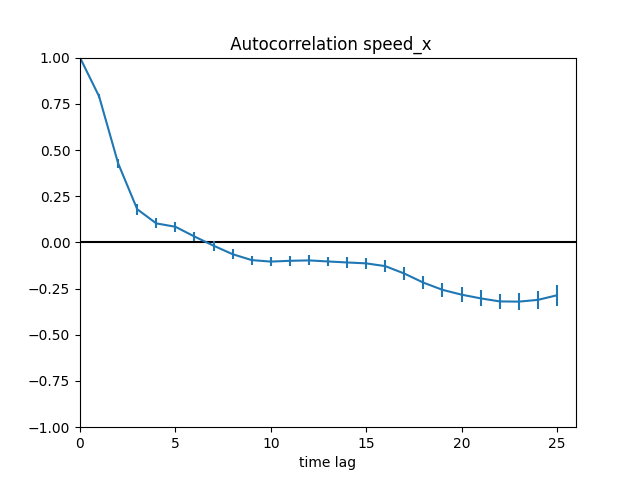
\includegraphics[width=\linewidth]{figures/acf_figures/glass_speed_x_acf_avg.png}
      \caption{Autocorrelation for speed x on glass}
    \end{subfigure}
    \begin{subfigure}[b]{0.4\linewidth}
      \includegraphics[width=\linewidth]{figures/acf_figures/stiff_speed_x_acf_avg.png}
      \caption{Autocorrelation for speed x on gel}
    \end{subfigure}
    \caption{These are different}
    \label{fig:acf_speedx}
  \end{figure}

\item Figure 8
\begin{figure}[h!]
    \centering
    \begin{subfigure}[b]{0.4\linewidth}
      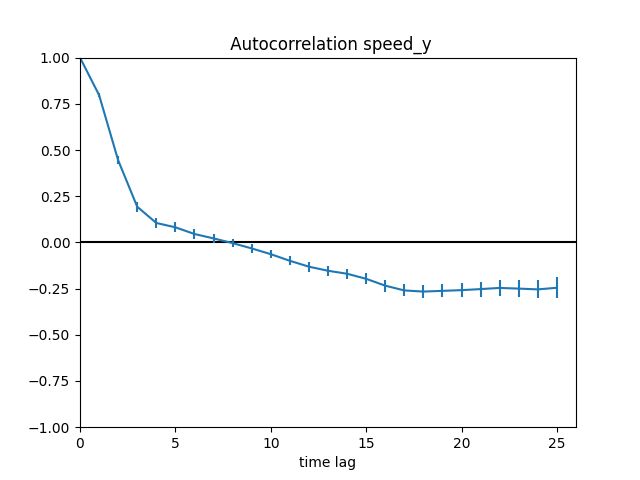
\includegraphics[width=\linewidth]{figures/acf_figures/glass_speed_y_acf_avg.png}
      \caption{Autocorrelation for speed y on glass}
    \end{subfigure}
    \begin{subfigure}[b]{0.4\linewidth}
      \includegraphics[width=\linewidth]{figures/acf_figures/stiff_speed_y_acf_avg.png}
      \caption{Autocorrelation for speed y on gel}
    \end{subfigure}
    \caption{These are different}
    \label{fig:acf_speedy}
  \end{figure}

\end{enumerate}

\end{document}
